% ============================================================
% 讲义 — 人教版八年级上册 第13章 轴对称
% 编译命令：xelatex -interaction=nonstopmode 第13章_轴对称.tex
% ============================================================
\documentclass[12pt, a4paper]{ctexart}
\usepackage[margin=2.2cm]{geometry}
\usepackage{amsmath, amssymb}
\usepackage{enumitem}
\usepackage{tcolorbox}
\usepackage{booktabs}
\usepackage{array}
\usepackage{fancyhdr}
\usepackage{xcolor}
\usepackage{tikz}
\usepackage{hyperref}
\usepackage{graphicx}
\usepackage{multirow}
\usepackage{pgfplots}
\pgfplotsset{compat=1.18}

% 颜色定义
\definecolor{mainblue}{RGB}{41, 98, 168}
\definecolor{lightblue}{RGB}{230, 240, 255}
\definecolor{tipgreen}{RGB}{34, 139, 87}
\definecolor{lightgreen}{RGB}{235, 250, 240}
\definecolor{warnred}{RGB}{200, 50, 50}
\definecolor{lightred}{RGB}{255, 240, 240}
\definecolor{examorange}{RGB}{210, 120, 20}
\definecolor{lightorange}{RGB}{255, 248, 235}
\definecolor{apppurple}{RGB}{120, 60, 170}
\definecolor{lightpurple}{RGB}{245, 238, 255}

% 页眉页脚
\pagestyle{fancy}
\fancyhf{}
\fancyhead[L]{\small\textcolor{mainblue}{\textbf{人教版八年级上册 · 第13章 轴对称}}}
\fancyhead[R]{\small\textcolor{mainblue}{轴对称讲义}}
\fancyfoot[C]{\small —\ \thepage\ —}
\renewcommand{\headrulewidth}{0.6pt}
\renewcommand{\headrule}{\hbox to\headwidth{\color{mainblue}\leaders\hrule height \headrulewidth\hfill}}
\renewcommand{\footrulewidth}{0pt}

% tcolorbox 样式
\newtcolorbox{knowledgebox}[1][]{%
  colback=lightblue, colframe=mainblue,
  fonttitle=\bfseries\large, title=#1,
  arc=3mm, boxrule=0.8pt,
  left=8pt, right=8pt, top=6pt, bottom=6pt
}

\newtcolorbox{tipbox}[1][]{%
  colback=lightgreen, colframe=tipgreen,
  fonttitle=\bfseries, title=#1,
  arc=2mm, boxrule=0.6pt,
  left=6pt, right=6pt, top=4pt, bottom=4pt
}

\newtcolorbox{warnbox}[1][]{%
  colback=lightred, colframe=warnred,
  fonttitle=\bfseries, title=#1,
  arc=2mm, boxrule=0.6pt,
  left=6pt, right=6pt, top=4pt, bottom=4pt
}

\newtcolorbox{examplebox}[1][]{%
  colback=lightorange, colframe=examorange,
  fonttitle=\bfseries, title=#1,
  arc=3mm, boxrule=0.8pt,
  left=8pt, right=8pt, top=6pt, bottom=6pt
}

\newtcolorbox{appbox}[1][]{%
  colback=lightpurple, colframe=apppurple,
  fonttitle=\bfseries, title=#1,
  arc=3mm, boxrule=0.8pt,
  left=8pt, right=8pt, top=6pt, bottom=6pt
}

\setCJKmainfont{Hiragino Sans GB}
\setCJKsansfont{Heiti SC}

\begin{document}

% ============ 标题页 ============
\begin{center}
{\Huge\bfseries\textcolor{mainblue}{第13章\quad 轴对称}}\\[12pt]
{\Large\textcolor{gray}{讲\quad 义}}\\[8pt]
\rule{0.6\textwidth}{1pt}\\[8pt]
{\normalsize 适用：人教版\quad 八年级上册\quad |\quad 课时：4课时}
\end{center}
\vspace{10pt}

% ==============================================================
% 第一部分：知识点讲解
% ==============================================================
\section*{\textcolor{mainblue}{一、知识点讲解}}

% -------------------- 13.1 轴对称 --------------------
\subsection*{13.1\quad 轴对称}

\begin{knowledgebox}[轴对称图形]
如果一个平面图形沿一条直线折叠，直线两旁的部分能够互相重合，这个图形就叫做\textbf{轴对称图形}，这条直线就是它的\textbf{对称轴}。

常见的轴对称图形：
\begin{itemize}[nosep]
  \item 线段（对称轴：线段的垂直平分线以及线段本身所在直线）
  \item 角（对称轴：角平分线所在直线）
  \item 等腰三角形（对称轴：底边上的高/中线/顶角平分线所在直线）
  \item 等边三角形（对称轴：三条，分别是三条边上的高所在直线）
  \item 长方形（对称轴：两条，分别是对边中点连线）
  \item 正方形（对称轴：四条）
  \item 圆（对称轴：无数条，任意一条直径所在直线）
\end{itemize}
\end{knowledgebox}

\begin{knowledgebox}[两个图形成轴对称]
把一个图形沿着某一条直线折叠，如果它能够与另一个图形重合，那么就说这两个图形\textbf{关于这条直线对称}（即两个图形成轴对称），这条直线叫做\textbf{对称轴}，折叠后重合的点是\textbf{对应点}（对称点）。
\end{knowledgebox}

\begin{warnbox}[易错辨析：轴对称图形 vs 两个图形成轴对称]
\begin{itemize}[nosep]
  \item \textbf{轴对称图形}是指\emph{一个}图形自身的对称性。
  \item \textbf{两个图形成轴对称}是指\emph{两个}图形之间的位置关系。
  \item 两者的联系：都沿某条直线折叠后重合；把成轴对称的两个图形看作一个整体，它就是一个轴对称图形。
\end{itemize}
\end{warnbox}

\begin{knowledgebox}[轴对称的性质]
\begin{enumerate}[nosep]
  \item 关于某条直线对称的两个图形是全等形（对应线段相等、对应角相等）。
  \item 如果两个图形关于某直线对称，那么对称轴是对应点连线的\textbf{垂直平分线}。
  \item 两个图形关于某直线对称，如果对应线段或其延长线相交，那么交点在对称轴上。
\end{enumerate}

\textbf{核心性质：}对应点连线被对称轴垂直平分。
\end{knowledgebox}

\tikzset{every picture/.style={line width=0.75pt}} % set default line width

\begin{center}
\begin{tikzpicture}[x=1cm, y=1cm]
  % 对称轴
  \draw[dashed, thick, blue] (0,-1.5) -- (0,3.5) node[above]{$l$（对称轴）};
  % 左侧三角形
  \coordinate (A) at (-2.5, 0);
  \coordinate (B) at (-1, 2.5);
  \coordinate (C) at (-1, 0);
  \draw[thick, red] (A) -- (B) -- (C) -- cycle;
  \node[left] at (A) {$A$};
  \node[left] at (B) {$B$};
  \node[below left] at (C) {$C$};
  % 右侧三角形
  \coordinate (A') at (2.5, 0);
  \coordinate (B') at (1, 2.5);
  \coordinate (C') at (1, 0);
  \draw[thick, red] (A') -- (B') -- (C') -- cycle;
  \node[right] at (A') {$A'$};
  \node[right] at (B') {$B'$};
  \node[below right] at (C') {$C'$};
  % 对应点连线
  \draw[dotted, gray] (A) -- (A');
  \draw[dotted, gray] (B) -- (B');
  \draw[dotted, gray] (C) -- (C');
  % 垂直平分标记
  \node[below, font=\small] at (0, -0.5) {$l$ 垂直平分 $AA'$、$BB'$、$CC'$};
\end{tikzpicture}
\end{center}

\begin{tipbox}[性质总结]
在轴对称中，找对称轴的方法：连接对应点，作对应点连线的垂直平分线，即为对称轴。
\end{tipbox}

% -------------------- 13.2 线段垂直平分线 --------------------
\subsection*{13.2\quad 线段垂直平分线}

\begin{knowledgebox}[线段垂直平分线的性质]
\textbf{定理：}线段垂直平分线上的点与这条线段两个端点的距离相等。

\medskip
即：若点 $P$ 在线段 $AB$ 的垂直平分线上，则 $PA = PB$。
\end{knowledgebox}

\begin{center}
\begin{tikzpicture}[scale=1.2]
  \coordinate (A) at (-2,0);
  \coordinate (B) at (2,0);
  \coordinate (M) at (0,0);
  \coordinate (P) at (0,2);
  \draw[thick] (A) -- (B);
  \draw[thick, blue] (P) -- (M);
  \draw[dashed, red] (P) -- (A) node[midway, left]{$=$};
  \draw[dashed, red] (P) -- (B) node[midway, right]{$=$};
  \node[below] at (A) {$A$};
  \node[below] at (B) {$B$};
  \node[below right] at (M) {$M$};
  \node[above left] at (P) {$P$};
  \node[below, font=\small] at (0,-0.6) {$l$（$AB$ 的垂直平分线）};
  \draw[blue, thick] (0,-0.4) -- (0,2.3);
  \node[left, font=\small, blue] at (0,1) {$\perp$};
\end{tikzpicture}
\end{center}

\begin{knowledgebox}[线段垂直平分线的判定]
\textbf{逆定理（判定）：}与一条线段两个端点距离相等的点，在这条线段的垂直平分线上。

\medskip
即：若 $PA = PB$，则点 $P$ 在线段 $AB$ 的垂直平分线上。
\end{knowledgebox}

\begin{tipbox}[与角平分线对比]
\begin{itemize}[nosep]
  \item 角平分线上的点到角两边的距离相等（角平分线性质）。
  \item 线段垂直平分线上的点到线段两端点的距离相等（垂直平分线性质）。
  \item 两者都是"距离相等"的几何表达，但场景不同。
\end{itemize}
\end{tipbox}

% -------------------- 13.3 等腰三角形 --------------------
\subsection*{13.3\quad 等腰三角形}

\begin{knowledgebox}[等腰三角形的性质]
\textbf{性质1（等边对等角）：}等腰三角形的两个底角相等（简称"等边对等角"）。

\medskip
即：在 $\triangle ABC$ 中，若 $AB = AC$，则 $\angle B = \angle C$。

\textbf{性质2（三线合一）：}等腰三角形的顶角平分线、底边上的中线、底边上的高互相重合。

\medskip
即：若 $AB = AC$，$AD$ 是顶角平分线，则 $AD$ 也是底边中线和底边上的高。

\textbf{性质3：}等腰三角形是轴对称图形，对称轴是底边上的高所在直线。
\end{knowledgebox}

\begin{center}
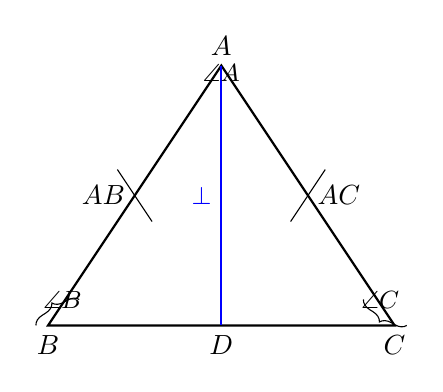
\begin{tikzpicture}[scale=1.1]
  \coordinate (A) at (0, 3);
  \coordinate (B) at (-2, 0);
  \coordinate (C) at (2, 0);
  \coordinate (D) at (0, 0);
  \draw[thick] (A) -- (B) -- (C) -- cycle;
  \draw[thick, blue] (A) -- (D);
  % 标记等边
  \node[left] at (-1, 1.5) {$AB$};
  \node[right] at (1, 1.5) {$AC$};
  \draw[mark=|] (-1.2, 1.8) -- (-0.8, 1.2);
  \draw[mark=|] (1.2, 1.8) -- (0.8, 1.2);
  % 标记角
  \node[left, font=\small] at (-1.5, 0.3) {$\angle B$};
  \node[right, font=\small] at (1.5, 0.3) {$\angle C$};
  \node[above, font=\small] at (0, 2.7) {$\angle A$};
  % 标记垂直
  \node[left, font=\small, blue] at (0, 1.5) {$\perp$};
  % 标记中点
  \node[below] at (D) {$D$};
  % 标记等角
  \draw[decorate, decoration={brace, amplitude=4pt}, xshift=-4pt] (-2,0) -- (-1.5,0.3);
  \draw[decorate, decoration={brace, amplitude=4pt}, xshift=4pt] (2,0) -- (1.5,0.3);
  \node[below] at (B) {$B$};
  \node[below] at (C) {$C$};
  \node[above] at (A) {$A$};
\end{tikzpicture}
\end{center}

\begin{knowledgebox}[等腰三角形的判定]
\textbf{判定（等角对等边）：}如果一个三角形有两个角相等，那么这两个角所对的边也相等（简称"等角对等边"）。

\medskip
即：在 $\triangle ABC$ 中，若 $\angle B = \angle C$，则 $AB = AC$，即 $\triangle ABC$ 是等腰三角形。
\end{knowledgebox}

\begin{warnbox}[易错提醒："等边对等角"与"等角对等边"]
\begin{itemize}[nosep]
  \item "等边对等角"是\textbf{性质}（已知等腰，推出底角相等）。
  \item "等角对等边"是\textbf{判定}（已知两角相等，推出等腰）。
  \item 使用时一定要写清楚依据，不能直接跳步。
\end{itemize}
\end{warnbox}

% -------------------- 等边三角形 --------------------
\subsection*{13.4\quad 等边三角形}

\begin{knowledgebox}[等边三角形的性质]
等边三角形（正三角形）是特殊的等腰三角形，三边相等。
\begin{enumerate}[nosep]
  \item 三条边相等，三个角都等于 $60°$。
  \item 每条边上的中线、高、对应角的角平分线互相重合（三线合一），共三条。
  \item 是轴对称图形，有三条对称轴。
\end{enumerate}
\end{knowledgebox}

\begin{knowledgebox}[等边三角形的判定]
\begin{enumerate}[nosep]
  \item 三条边都相等的三角形是等边三角形（定义）。
  \item 三个角都等于 $60°$ 的三角形是等边三角形。
  \item 有一个角等于 $60°$ 的等腰三角形是等边三角形。
\end{enumerate}
\end{knowledgebox}

% -------------------- 最短路径 --------------------
\subsection*{13.5\quad 最短路径问题（将军饮马模型）}

\begin{knowledgebox}[将军饮马问题]
\textbf{问题：}在直线 $l$ 的同侧有两个点 $A$、$B$，在直线 $l$ 上找一点 $P$，使 $PA + PB$ 最小。

\textbf{方法：}
\begin{enumerate}[nosep]
  \item 作点 $A$ 关于直线 $l$ 的对称点 $A'$；
  \item 连接 $A'B$，与直线 $l$ 的交点即为所求点 $P$；
  \item 此时 $PA + PB = PA' + PB = A'B$（两点之间线段最短）。
\end{enumerate}
\end{knowledgebox}

\begin{center}
\begin{tikzpicture}[scale=1.0]
  % 直线
  \draw[thick, blue] (-1,0) -- (7,0) node[right]{$l$};
  % 点A在上方
  \coordinate (A) at (1, 2.5);
  \coordinate (B) at (5, 2);
  % A的对称点A'
  \coordinate (Aprime) at (1, -2.5);
  % P点
  \coordinate (P) at (2.28, 0);
  % 画点
  \fill (A) circle (2pt) node[above]{$A$};
  \fill (B) circle (2pt) node[above]{$B$};
  \fill (Aprime) circle (2pt) node[below]{$A'$};
  \fill (P) circle (2pt) node[below]{$P$};
  % AP, PB
  \draw[thick, red] (A) -- (P) -- (B);
  % A'P (dashed)
  \draw[dashed, gray] (Aprime) -- (P);
  % A到l的垂线
  \draw[dotted, gray] (A) -- (1,0);
  \draw[dotted, gray] (Aprime) -- (1,0);
  % 垂直标记
  \node[left, font=\small, gray] at (1, 1.25) {$\perp$};
\end{tikzpicture}
\end{center}

\begin{tipbox}[最短路径问题的解题思路]
遇到"距离之和最小"的问题，通常利用\textbf{对称变换}将折线段转化为直线段，再利用"两点之间线段最短"来求解。关键步骤是"作对称点、连线、找交点"。
\end{tipbox}

% ==============================================================
% 第二部分：例题精讲
% ==============================================================
\section*{\textcolor{examorange}{二、例题精讲}}

\begin{examplebox}[【例题1】基础计算——利用等腰三角形求角]
在等腰三角形 $ABC$ 中，$AB = AC$，$\angle A = 40°$，求 $\angle B$ 和 $\angle C$ 的度数。
\end{examplebox}

\textbf{解：}

因为 $AB = AC$（已知），所以 $\triangle ABC$ 是等腰三角形。

由"等边对等角"得：$\angle B = \angle C$。

又因为三角形内角和为 $180°$，所以
$$\angle B + \angle C = 180° - \angle A = 180° - 40° = 140°$$

因此 $\angle B = \angle C = \dfrac{140°}{2} = 70°$。

\begin{tipbox}[方法总结]
等腰三角形求角的基本思路：利用"等边对等角"列出等量关系，再结合三角形内角和定理（$180°$）列方程求解。注意讨论顶角和底角两种情况。
\end{tipbox}

\begin{examplebox}[【例题2】等腰三角形的存在性——分类讨论]
已知等腰三角形的一边长为 $4$，另一边长为 $9$，求该等腰三角形的周长。
\end{examplebox}

\textbf{解：}

需要分两种情况讨论：

\textbf{情况一：}腰长为 $4$，底边为 $9$。

此时三边为 $4, 4, 9$。检验：$4 + 4 = 8 < 9$，不满足三角形三边关系（两边之和大于第三边），所以这种情况不成立。

\textbf{情况二：}腰长为 $9$，底边为 $4$。

此时三边为 $9, 9, 4$。检验：$9 + 4 = 13 > 9$，$9 + 9 = 18 > 4$，满足三边关系，成立。

所以该等腰三角形的周长 $= 9 + 9 + 4 = 22$。

\begin{tipbox}[方法总结]
等腰三角形边长问题一定要\textbf{分类讨论}（腰和底边分别是什么），讨论后要\textbf{验证三边关系}（任意两边之和大于第三边），排除不成立的情况。
\end{tipbox}

\begin{examplebox}[【例题3】证明题——等角对等边的判定应用]
已知：如图，在 $\triangle ABC$ 中，$\angle B = \angle C$。求证：$AB = AC$。
\end{examplebox}

\textbf{已知：}在 $\triangle ABC$ 中，$\angle B = \angle C$。

\textbf{求证：}$AB = AC$。

\textbf{证明：}

作 $BC$ 边上的高 $AD$（$D$ 在 $BC$ 上），则 $\angle ADB = \angle ADC = 90°$。

在 $\triangle ABD$ 和 $\triangle ACD$ 中：
$$\left\{\begin{array}{l}
\angle ADB = \angle ADC = 90° \\
\angle B = \angle C \quad \text{（已知）} \\
AD = AD \quad \text{（公共边）}
\end{array}\right.$$

由"AAS"（或"角角边"）判定定理，$\triangle ABD \cong \triangle ACD$。

所以 $AB = AC$（全等三角形对应边相等）。

即 $\triangle ABC$ 是等腰三角形。

\begin{tipbox}[方法总结]
"等角对等边"的证明方法：通过作辅助线（高线），构造两个直角三角形全等，从而得出对应边相等。这是证明等腰三角形的标准方法。
\end{tipbox}

\begin{examplebox}[【例题4】垂直平分线性质的综合应用]
在 $\triangle ABC$ 中，$AB$ 的垂直平分线交 $BC$ 于点 $D$，连接 $AD$。若 $BC = 10$，$AC = 6$，求 $\triangle ADC$ 的周长。
\end{examplebox}

\textbf{解：}

因为 $D$ 在 $AB$ 的垂直平分线上，由线段垂直平分线的性质得：
$$DA = DB$$

$\triangle ADC$ 的周长 $= AD + DC + AC = DB + DC + AC = BC + AC$。

又因为 $BC = 10$，$AC = 6$，所以
$$\triangle ADC \text{ 的周长} = 10 + 6 = 16$$

\begin{tipbox}[方法总结]
垂直平分线上的点到线段两端距离相等，利用这一性质可以将折线段转化为直线段，从而方便计算周长。这类题的关键是识别"垂直平分线"条件并应用性质进行\textbf{等量代换}。
\end{tipbox}

\begin{examplebox}[【例题5】易错辨析——轴对称与全等的关系]
判断以下说法是否正确，并说明理由：

\textbf{(1)} 如果两个三角形全等，那么它们一定关于某条直线对称。

\textbf{(2)} 如果两个三角形关于某条直线对称，那么它们一定全等。
\end{examplebox}

\textbf{解：}

\textbf{(1)} 错误。

理由：全等三角形可以通过平移、旋转得到，不一定通过翻折（轴对称）得到。例如，将一个三角形向右平移一段距离后，两个三角形全等但不关于任何直线对称。

\textbf{(2)} 正确。

理由：轴对称的性质告诉我们，关于某条直线对称的两个图形是全等形，所以两个三角形如果关于某条直线对称，它们一定全等。

\begin{warnbox}[易错提醒]
\begin{itemize}[nosep]
  \item 全等 $\not\Rightarrow$ 轴对称（全等可以通过多种变换实现）。
  \item 轴对称 $\Rightarrow$ 全等（轴对称一定全等）。
  \item "轴对称"是比"全等"更强的条件，它还确定了两个图形的位置关系。
\end{itemize}
\end{warnbox}

\begin{examplebox}[【例题6】综合提高——将军饮马问题]
如图，牧马人从 $A$ 地出发，先到草地边 $l_1$ 喂马，再到河边 $l_2$ 饮马，然后回到 $B$ 地。$A$、$B$ 在两条平行线之间，$A$ 距 $l_1$ 为 $2$ km，$B$ 距 $l_2$ 为 $3$ km，$A$、$B$ 水平距离为 $6$ km，$l_1$ 与 $l_2$ 的距离为 $10$ km。求最短路径的长度。
\end{examplebox}

\textbf{解：}

建立坐标系：设 $l_1$ 为 $y = 0$，$l_2$ 为 $y = -10$。

则 $A = (0, 2)$，$B = (6, -7)$（因为 $B$ 距 $l_2$ 为 $3$，所以在 $l_2$ 上方 $3$ 处，即 $y = -10 + 3 = -7$）。

\textbf{第一步：}作 $A$ 关于 $l_1$ 的对称点 $A'$，$A' = (0, -2)$。

\textbf{第二步：}作 $B$ 关于 $l_2$ 的对称点 $B'$，$B' = (6, -13)$。

\textbf{第三步：}连接 $A'B'$，$A'B'$ 与 $l_1$ 的交点为 $M$，与 $l_2$ 的交点为 $N$。

则最短路径为 $A \to M \to N \to B$，长度等于 $A'B'$ 的长度。

$$A'B' = \sqrt{(6-0)^2 + (-13-(-2))^2} = \sqrt{36 + 121} = \sqrt{157} \text{ (km)}$$

\begin{tipbox}[方法总结]
"两次对称"将军饮马问题的解法：
\begin{enumerate}[nosep]
  \item 分别作起点和终点关于各自直线的对称点；
  \item 连接两个对称点，连线与两条直线的交点即为最优拐点；
  \item 最短路径长度等于两个对称点之间的距离。
\end{enumerate}
本质是将折线段通过两次对称变换拉直为直线段。
\end{tipbox}

\begin{examplebox}[【例题7】交叉综合——轴对称与三角形全等综合]
已知：如图，在 $\triangle ABC$ 中，$AB = AC$，$D$ 是 $BC$ 上的一点，$DE \perp AB$ 于 $E$，$DF \perp AC$ 于 $F$。求证：$DE + DF$ 等于定值（等于 $AB$ 边上的高）。
\end{examplebox}

\textbf{已知：}$AB = AC$，$DE \perp AB$，$DF \perp AC$，$D$ 在 $BC$ 上。

\textbf{求证：}$DE + DF = h$（$h$ 为 $AB$ 边上的高，即 $BC$ 边上的高）。

\textbf{证明：}

作 $AH \perp BC$ 于 $H$（$H$ 在 $BC$ 上），则 $AH = h$。

连接 $AD$，则 $S_{\triangle ABC} = S_{\triangle ABD} + S_{\triangle ADC}$。

由面积公式：
$$\frac{1}{2} \cdot BC \cdot AH = \frac{1}{2} \cdot AB \cdot DE + \frac{1}{2} \cdot AC \cdot DF$$

因为 $AB = AC$，化简得：
$$\frac{BC \cdot AH}{AB} = DE + DF$$

又因为在等腰三角形中 $BC$ 和 $AH$ 为定值，$AB$ 也为定值，所以 $DE + DF$ 为定值。

\begin{tipbox}[方法总结]
涉及等腰三角形上一点到两腰距离之和（或差）的问题，常用\textbf{面积法}来解决。通过将大三角形的面积拆分为两个小三角形面积之和，利用等腰三角形两腰相等的条件，建立等量关系。这是面积法的经典应用。
\end{tipbox}

% ==============================================================
% 第三部分：应用题
% ==============================================================
\section*{\textcolor{apppurple}{三、应用题}}

\begin{appbox}[【应用1】镜面对称——镜中时钟]
小明在镜子中看到时钟显示为 $2:50$，请问实际时间是几点几分？
\end{appbox}

\textbf{解：}

镜子中的像与实物关于镜面（竖直方向的对称轴）成轴对称。在镜子中，时针和分针的位置是左右翻转的。

\textbf{方法：}用 $12:00$ 减去镜子中看到的时间。

$$12:00 - 2:50 = 9:10$$

所以实际时间是 \textbf{9点10分}。

验证：9:10时，时针在9和10之间、分针指向2（即10分钟的位置），左右翻折后时针在2和3之间、分针指向10（即50分钟的位置），在镜中显示为 $2:50$，符合。

\begin{tipbox}[方法总结]
镜面时钟问题利用轴对称原理：实际时间 $+$ 镜中时间 $= 12:00$。记住这个规律可以快速求解。
\end{tipbox}

\begin{appbox}[【应用2】光学反射——光路最短问题]
一束光线从点 $A(1, 3)$ 出发，射到 $x$ 轴上的点 $P$ 后反射，反射光线经过点 $B(5, 1)$。求点 $P$ 的坐标。（入射角 $=$ 反射角）
\end{appbox}

\textbf{解：}

根据光学反射定律（入射角 $=$ 反射角），反射问题等价于轴对称问题。

\textbf{第一步：}作 $A$ 关于 $x$ 轴的对称点 $A'$。$A = (1, 3)$，所以 $A' = (1, -3)$。

\textbf{第二步：}连接 $A'B$，$A'B$ 与 $x$ 轴的交点即为 $P$。

直线 $A'B$ 过点 $(1, -3)$ 和 $(5, 1)$：
$$\text{斜率} = \frac{1-(-3)}{5-1} = \frac{4}{4} = 1$$

直线方程：$y - (-3) = 1 \cdot (x - 1)$，即 $y = x - 4$。

令 $y = 0$（$x$ 轴），得 $x = 4$。

所以 $P = (4, 0)$。

\begin{tipbox}[方法总结]
光的反射问题利用轴对称原理：入射角等于反射角 $\Leftrightarrow$ 光线关于反射面成轴对称。解法与将军饮马模型一致：作对称点、连线、找交点。
\end{tipbox}

\begin{appbox}[【应用3】等腰三角形在建筑中的应用——人字形屋顶]
如图，一栋房屋的人字形屋顶 $ABC$ 中，$AB = AC$，屋顶的跨度 $BC = 8$ 米，屋脊到横梁的垂直距离（即 $BC$ 边上的高）$AD = 3$ 米。求屋顶两侧斜面的长度 $AB$（即腰长）。
\end{appbox}

\textbf{解：}

因为 $AB = AC$，所以 $\triangle ABC$ 是等腰三角形。

$AD$ 是 $BC$ 边上的高，由等腰三角形"三线合一"的性质，$D$ 是 $BC$ 的中点。

所以 $BD = DC = \dfrac{BC}{2} = \dfrac{8}{2} = 4$（米）。

在直角三角形 $ABD$ 中，由勾股定理：
$$AB = \sqrt{AD^2 + BD^2} = \sqrt{3^2 + 4^2} = \sqrt{9 + 16} = \sqrt{25} = 5 \text{ (米)}$$

所以屋顶两侧斜面的长度 $AB = AC = 5$ 米。

\begin{tipbox}[方法总结]
等腰三角形在建筑中应用广泛。利用"三线合一"性质可以将等腰三角形转化为直角三角形，再用勾股定理求解。实际问题中常需要求腰长、底边长或高。
\end{tipbox}

% ==============================================================
% 第四部分：课堂练习
% ==============================================================
\section*{\textcolor{tipgreen}{四、课堂练习}}

\begin{enumerate}
  \item 等腰三角形的一个角为 $50°$，求另外两个角的度数。

  \item 在 $\triangle ABC$ 中，$AB = AC$，$BD$ 平分 $\angle ABC$，$\angle BDC = 75°$，求 $\angle A$ 的度数。

  \item 如图，$AD$ 是 $\triangle ABC$ 中 $BC$ 边的垂直平分线，$AB = 5$，$AC = 3$，求 $\triangle ADC$ 的周长。

  \item 已知等腰三角形的底边长为 $6$，腰上的高为 $4$，求腰长。

  \item 在直线 $l$ 的同侧有两点 $A$、$B$，$A$ 到 $l$ 的距离为 $2$，$B$ 到 $l$ 的距离为 $5$，$A$、$B$ 的水平距离为 $6$。在直线 $l$ 上求一点 $P$，使 $PA + PB$ 最小，并求最小值。
\end{enumerate}

\vspace{10pt}

\begin{knowledgebox}[参考答案]

\textbf{第1题：}

情况一：$50°$ 为顶角，则底角 $= \dfrac{180° - 50°}{2} = 65°$，另外两角为 $65°$、$65°$。

情况二：$50°$ 为底角，则另一个底角 $= 50°$，顶角 $= 180° - 50° - 50° = 80°$，另外两角为 $50°$、$80°$。

\medskip
\textbf{第2题：}

设 $\angle ABD = \angle DBC = x$，则 $\angle ABC = 2x$。

在 $\triangle BDC$ 中：$\angle BDC + \angle DCB + \angle DBC = 180°$。

又 $\angle BDC = 75°$，$\angle DCB = \angle ABC = 2x$（等边对等角），$\angle DBC = x$。

所以 $75° + 2x + x = 180°$，$3x = 105°$，$x = 35°$。

$\angle ABC = 2x = 70°$，$\angle C = 70°$。

$\angle A = 180° - 70° - 70° = 40°$。

\medskip
\textbf{第3题：}

$D$ 在 $BC$ 的垂直平分线上，所以 $DB = DC$。

$\triangle ADC$ 的周长 $= AD + DC + AC = AD + DB + AC = AB + AC = 5 + 3 = 8$。

\medskip
\textbf{第4题：}

设腰长为 $a$，底边 $BC = 6$，腰上的高 $h = 4$。

由面积法：$S = \frac{1}{2} \cdot 6 \cdot h_{BC} = \frac{1}{2} \cdot a \cdot 4$。

设 $BC$ 边上的高为 $h_{BC}$，则 $h_{BC} = \sqrt{a^2 - 9}$。

由 $\frac{1}{2} \cdot 6 \cdot \sqrt{a^2 - 9} = \frac{1}{2} \cdot a \cdot 4$，得 $3\sqrt{a^2 - 9} = 2a$。

两边平方：$9(a^2 - 9) = 4a^2$，$5a^2 = 81$，$a^2 = \dfrac{81}{5}$，$a = \dfrac{9}{\sqrt{5}} = \dfrac{9\sqrt{5}}{5}$。

\medskip
\textbf{第5题：}

建立坐标系，设 $l$ 为 $x$ 轴。$A = (0, 2)$，$B = (6, 5)$。

作 $A$ 关于 $x$ 轴的对称点 $A' = (0, -2)$。

连接 $A'B$，$A'B = \sqrt{(6-0)^2 + (5-(-2))^2} = \sqrt{36 + 49} = \sqrt{85}$。

$A'B$ 的方程：斜率 $= \dfrac{7}{6}$，$y + 2 = \dfrac{7}{6}x$，令 $y = 0$ 得 $x = \dfrac{12}{7}$。

$P = \left(\dfrac{12}{7}, 0\right)$，$PA + PB$ 的最小值 $= \sqrt{85}$。

\end{knowledgebox}

\vfill
\begin{center}
\small\textcolor{gray}{本讲义仅供教学参考，例题可根据学生水平调整难度。}
\end{center}

\end{document}
